\chapter{Vérification des critères}
% D'après le sujet, pour chaque critère :
% - Jeux de tests satisfaisant et ne satisfaisant pas le critère
% - Mécanisme de vérification
% - Mécanisme de génération
% Et en général : relations d'ordre entre les critères

\section{Toutes les affectations}
\label{sec:affectations}
On va travailler sur le programme suivant :

\begin{minipage}{0.46\textwidth}
\begin{verbatim}
1:  if (X <= 0) {
2:      X := -X;
    } else {
3:      X := 1 - X;
    }

4:  if (X == 1) {
5:      X := 1;
    } else {
6:      X := X + 1;
    }
\end{verbatim}
\end{minipage}
\begin{minipage}{0.46\textwidth}
	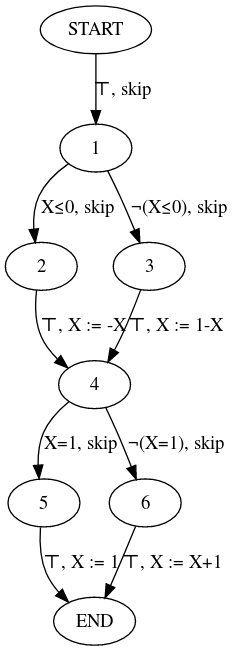
\includegraphics[scale=0.5]{pics/simpleCFG.png}
	\captionof{figure}{CFG associé}
\end{minipage}

%Ajouter AST + CFG en illustration de la partie précédente

Le critère \textit{Toutes les affectations} demande à ce que tous les labels d'affectations (ici : $2, 3, 5, 6$) apparaissent au moins une fois dans l'un des chemins d'exécution correspondant aux données de tests.

Si on prend pour jeu de test :

\[ \{
	\{ X : -1\},
	\{ X : 1\}
\} \]

On obtient les chemins d'exécutions suivants :
\begin{description}
\item[$\{ X : -1\}$ : ] $1, 2, 4, 5$
\item[$\{ X : 1\}$ : ] $1, 3, 4, 6$
\end{description}

On est donc passé au moins une fois par chaque label associé à une affectation : le critère est vérifié sur ce programme et ce jeu de test.

Si, en revanche, on s'était contenté d'un unique test $\{ X : -1\}$, on ne serait pas passé par les noeuds $3$ et $6$, et le critère n'aurait pas été vérifié.

Dans la pratique, étant donné un CFG, on récupère l'ensemble des noeuds (labels) tels qu'une arête sortante de ce noeud porte une affectation. Ceci se fait très facilement en parcourant l'ensemble des arêtes (sans notion de chemin ici).
Il suffit ensuite de regarder lesquels de ces noeuds sont (ou non) dans les chemins des tests.

\section{Toutes les décisions}

On travaille toujours sur le programme défini en \ref{sec:affectations}.

Le critère \textit{Toutes les décisions} demande à ce que l'on passe au moins une fois par toutes les arêtes associées à une expression booléenne. Il s'agit, en bref, de toutes les arêtes sortantes des noeuds \textit{if} et \textit{while}, ce qui est équivalent à dire qu'il faut passer par les noeuds de destination de ces arêtes.

Ici, il faut donc passer par les noeuds $2, 3, 5, 6$. On retombe dans ce cas très simple sur les même éléments que le critère \textit{Toutes les affectations}, et le même jeu de tests vérifie donc les deux critères.

\section{Tous les \textit{k}-chemins}

Ce critère demande que chaque chemin d'exécution de longueur inférieure ou égale à $k$ soit exécuté.

On commence donc par implémenter un générateur qui va renvoyer tous les chemins correspondants. Pour ce faire, on réalise un parcours en profondeur du graphe, où l'on s'arête lorsqu'on à un chemin complet (noeud \textit{END} atteint) ou lorsque l'on a atteint la longueur maximale $k$.

Une fois que l'on a l'ensemble des chemins à vérifier, il suffit de comparer cet ensemble avec celui des chemins exécutés par les tests.

Sur le programme de la partie \ref{sec:affectations}, pour le critère \textit{Tous les 10-chemins}, il faut vérifier les chemins suivants (en fait, tous, car on a pris $k$ grand):

\begin{align*}
\{
	&[START, 1, 2, 4, 5, END],\\
	&[START, 1, 2, 4, 6, END],\\
	&[START, 1, 3, 4, 5, END],\\
	&[START, 1, 3, 4, 6, END]
\}
\end{align*}

On note que le chemin $[START, 1, 3, 4, 5, END]$ n'est pas faisable. Malheureusement, cela ne peut se détecter qu'à l'étape de génération des tests  : d'où l'importance de signaler à l'utilisateur quels sont les chemins manquants afin qu'il puisse décider de lui-même si ou non la couverture peut-être améliorée en complétant le jeu de tests.

Le jeu de tests suivant permet d'atteindre la couverture maximale :

\[ \{
	\{ X : -1\},
	\{ X : 1\};
	\{ X : 3\},
\} \]


\section{Toutes les \textit{i}-boucles}

On cherche ici tous les chemins pour lesquels les boucles while sont exécutées au plus $i$ fois. Attention, les "compteurs" des boucles imbriquées internes doivent être remis à zéro à chaque itération de la boucle externe. Le critère peut aussi se formuler "tous les chemins pour lesquels les boucles whiles sont exécutées au plus $i$ fois \textbf{à la suite}.

Sur le même principe que les $k$-chemins, on réalisé un générateur de chemins d'intérêt basé sur un parcours en profondeur. On maintient cette fois un compteur par boucle, et on veille à réinitialiser les compteurs des boucles imbriquées internes lorsque c'est nécessaire.

Il suffit ensuite de comparer les chemins obtenus avec ceux des tests.

Voici un programme comportant une boucle :

\begin{minipage}{0.46\textwidth}
\begin{verbatim}
1:  if (x >= 0) {
2:      x := x + 1;
    } else {
3:      x := x - 1;
4:      y := 3;
5:      z := y + 1;
    }

6:  while (z <= 0) {
7:      z := x + 1;
    }

8:  print(x);
\end{verbatim}
\end{minipage}
\begin{minipage}{0.46\textwidth}
	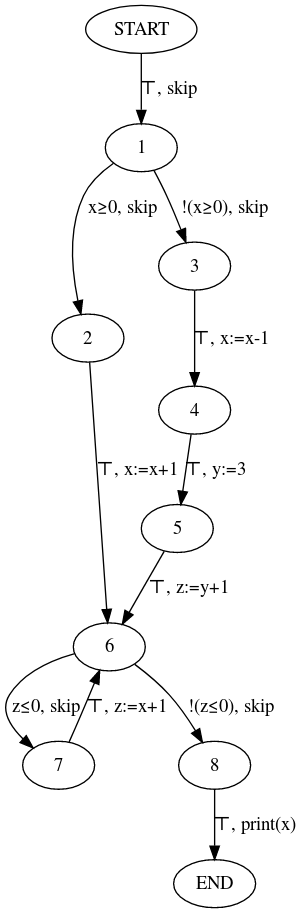
\includegraphics[scale=0.5]{pics/whileCFG.png}
	\captionof{figure}{CFG associé}
\end{minipage}

Les chemins à parcourir pour \textit{Toutes les 1-boucles} sont :

\begin{align*}
\{
&[START, 1, 2, 6, 8, END], \\
&[START, 1, 2, 6, 7, 6, 8, END], \\
&[START, 1, 3, 4, 5, 6, 8, END], \\
&[START, 1, 3, 4, 5, 6, 7, 6, 8, END] -> Infaisable
\}
\end{align*}

Le jeu de test suivant vérifie le critère :

\[ \{
	\{ X : -1, Z : 0\},
	\{ X : 0, Z : 0\};
	\{ X : 0, Z : 1\},
\} \]

\section{Toutes les définitions}

Le critère \textit{Toutes les définitions} demande que, pour chaque variable $X$, pour chaque noeud $u$ affectant $X$, on ait un chemin $..u...v..$ tel que $v$ utilise $X$, et qu'il n'y ait pas de réaffectation de $X$ entre $u$ et $v$.

Pour vérifier ce critère, nous commençons par implémenter les fonctions \textit{def} et \textit{ref} telles que définies dans l'énoncé.

On construit ensuite un dictionnaire \textit{definitions} qui associe à chaque variable $X$ l'ensemble des noeuds u tels que $X \in def(u)$.

Pour chaque variable $X$, on regarde ensuite chaque chemin. Si on trouve un noeud $u$ intéressant, c'est à dire $X \in def(u)$, on suit le chemin jusqu'à trouver $v$ tel que $X \in ref(v)$. On s'assure bien sûr qu'entre $u$ et $v$, il n'y a pas de noeud $u'$ tel que $X \in ref(u')$. Si on trouve $v$, on supprime $u$ de $\textit{definitions}[X]$.

Si à la fin, \textit{definitons} est vide, alors le critère est vérifié.

Le programme de la partie \ref{sec:affectations} ne pourra jamais vérifier ce critère, quel que soit le jeu de test, car les affectations $5$ et $6$ ne sont jamais utilisées. Si on rajoute une commande print qui affiche une variable, ainsi qu'une nouvelle variable $Y$, on peut le réécrire :


\begin{verbatim}
1:  if (X <= 0) {
2:      X := -X;
3:		Y := 5;
    } else {
4:      X := 1 - X;
    }

5:  if (X == 1) {
6:      X := 1;
    } else {
7:      X := X + 1;
8:		print(Y);
    }
9: print(X);
\end{verbatim}

Le dictionnaire \textit{definitions} s'écrit alors :

\[ \{
	X : [2, 4, 6, 7],
	Y : [3]
\} \]

Le jeu de tests suivant ne vérifie pas le critère :

\[ \{
	\{ X=1, Y=1\},
	\{ X=-1, Y=1 \}
\} \]

(Pas de chemin entre 3 et 8)


Contrairement à cet autre jeu de tests :

\[ \{
	\{ X=1, Y=1\},
	\{ X=-2, Y=1 \}
\} \]

\section{Toutes les utilisations}

Le critère \textit{Toutes les utilisations} demande que toutes ls utilisations acessibles pour chaque définitions soient exécutées au moins une fois.

On crée en parcourant le graphe un dictionnaire \textit{usages} qui pour chaque variable $X$, associe à chaque noeud $u$ définissant $X$ ($X \in def(u)$) l'ensemble des noeuds $v$ successeurs de $u$ tels que $v$ utilise $X$ ($X \in ref(v)$) tels qu'il n'y ait pas de noeud $u'$ qui redéfinisse X sur le chemin de $u$ à $v$.

On modifie le programme pour mieux montrer ce critère :
\begin{verbatim}
1:  if (X <= 0) {
2:      X := -X;
    } else {
3:      X := 1 - X;
    }

4:  if (X == 1) {
5:      X := 1;
    } else {
6:      X := X + 1;
7: 		print(X);
    }
\end{verbatim}

Le dictionnaire \textit{usages} s'écrit :

\begin{align*}
usages = \{
			X : \{ &\\
		&2 : 4, \\
		&3 : 4, \\
		&6 : 7,	\}\}
\end{align*}

Un jeu de test vérifiant ce critère pour ce programme est alors :

\begin{align*}
\{
	\{ X : 0 \},
	\{ X : 1 \}
\}
\end{align*}

Notons que contrairement au critère \textit{Toutes les définitions}, le critère \textit{Toutes les utilisations} n'impose pas l'existence d'une utilisation !

\section{Tous les DU-chemins}

Tous les chemins simples entre une définition de $X$ et une utilisation de $X$ sans redéfinition doivent être exécutés au moins une fois.

Le critère \textit{Toutes les utilisations} demandait simplement qu'au moins un chemin entre une paire (utilisation, définition) soit exécuté, ce critère-ci demande que tous les chemins simples le soient.

On récupère tous les chemins simples entre chaque noeud de définition ($def(u) \neq \emptyset$) et $END$ grâce à la librairie \textit{networkx}.

On regarde ensuite ces chemins à la recherche de paire $(u, v)$ telles que $u$ définit $X$, $v$ utilise $X$, et il n'y a pas de redéfinition de $X$ entre $u$ et $v$.

Lorsqu'on trouve une telle paire, on stocke le chemin entre $u$ et $v$ dans un dictionnaire \textit{du\_paths}.

Il suffit ensuite de chercher ces morceaux de chemins dans les chemins d'exécutions correspondants aux tests.

\section{Toutes les conditions}

Nous n'avons pas implémenté ce critère faute de temps. Il est toutefois possible de tirer parti de notre structure d'AST : on peut envisager qu'au moment de la conversion entre l'AST et le CFG on transforme chaque décision en un ensemble de noeuds \textit{If} correctement hiérarchisés. On pourrait ensuite vérifier le critère \textit{Toutes les décisions} sur ce nouveau CFG plus détaillé.